% Iterates q_{n+1} = G(q_n) from q_0 = 0 for two offspring laws: left, mean 3/4 (extinction certain); right, mean 5/4 (q = 1/2). Generated by a short script.
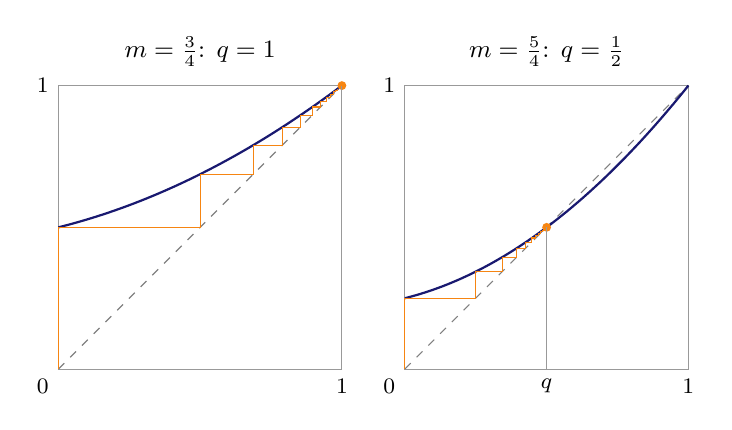
\begin{tikzpicture}
\begin{scope}[shift={(0,0)},x=3.6cm,y=3.6cm]
\draw[black!40] (0,0) rectangle (1,1);
\draw[black!50,dashed] (0,0)--(1,1);
\draw[MidnightBlue,thick] plot coordinates {(0.000,0.5000) (0.010,0.5025) (0.020,0.5051) (0.030,0.5077) (0.040,0.5104) (0.050,0.5131) (0.060,0.5159) (0.070,0.5187) (0.080,0.5216) (0.090,0.5245) (0.100,0.5275) (0.110,0.5305) (0.120,0.5336) (0.130,0.5367) (0.140,0.5399) (0.150,0.5431) (0.160,0.5464) (0.170,0.5497) (0.180,0.5531) (0.190,0.5565) (0.200,0.5600) (0.210,0.5635) (0.220,0.5671) (0.230,0.5707) (0.240,0.5744) (0.250,0.5781) (0.260,0.5819) (0.270,0.5857) (0.280,0.5896) (0.290,0.5935) (0.300,0.5975) (0.310,0.6015) (0.320,0.6056) (0.330,0.6097) (0.340,0.6139) (0.350,0.6181) (0.360,0.6224) (0.370,0.6267) (0.380,0.6311) (0.390,0.6355) (0.400,0.6400) (0.410,0.6445) (0.420,0.6491) (0.430,0.6537) (0.440,0.6584) (0.450,0.6631) (0.460,0.6679) (0.470,0.6727) (0.480,0.6776) (0.490,0.6825) (0.500,0.6875) (0.510,0.6925) (0.520,0.6976) (0.530,0.7027) (0.540,0.7079) (0.550,0.7131) (0.560,0.7184) (0.570,0.7237) (0.580,0.7291) (0.590,0.7345) (0.600,0.7400) (0.610,0.7455) (0.620,0.7511) (0.630,0.7567) (0.640,0.7624) (0.650,0.7681) (0.660,0.7739) (0.670,0.7797) (0.680,0.7856) (0.690,0.7915) (0.700,0.7975) (0.710,0.8035) (0.720,0.8096) (0.730,0.8157) (0.740,0.8219) (0.750,0.8281) (0.760,0.8344) (0.770,0.8407) (0.780,0.8471) (0.790,0.8535) (0.800,0.8600) (0.810,0.8665) (0.820,0.8731) (0.830,0.8797) (0.840,0.8864) (0.850,0.8931) (0.860,0.8999) (0.870,0.9067) (0.880,0.9136) (0.890,0.9205) (0.900,0.9275) (0.910,0.9345) (0.920,0.9416) (0.930,0.9487) (0.940,0.9559) (0.950,0.9631) (0.960,0.9704) (0.970,0.9777) (0.980,0.9851) (0.990,0.9925) (1.000,1.0000)};
\draw[BurntOrange,thin] (0.0000,0.0000)--(0.0000,0.5000)--(0.5000,0.5000)--(0.5000,0.6875)--(0.6875,0.6875)--(0.6875,0.7900)--(0.7900,0.7900)--(0.7900,0.8536)--(0.8536,0.8536)--(0.8536,0.8955)--(0.8955,0.8955)--(0.8955,0.9244)--(0.9244,0.9244)--(0.9244,0.9447)--(0.9447,0.9447)--(0.9447,0.9593)--(0.9593,0.9593)--(0.9593,0.9699)--(0.9699,0.9699)--(0.9699,0.9776)--(0.9776,0.9776)--(0.9776,0.9834)--(0.9834,0.9834)--(0.9834,0.9876)--(0.9876,0.9876);
\fill[BurntOrange] (1.0000,1.0000) circle (1.6pt);
\draw[black!40] (1.0000,0)--(1.0000,1.0000);
\node[below left,font=\footnotesize] at (0,0) {$0$};
\node[below,font=\footnotesize] at (1,0) {$1$};
\node[font=\small] at (0.5,1.12) {$m=\frac34$: $q=1$};
\node[left,font=\footnotesize] at (0,1) {$1$};
\end{scope}
\begin{scope}[shift={(4.4,0)},x=3.6cm,y=3.6cm]
\draw[black!40] (0,0) rectangle (1,1);
\draw[black!50,dashed] (0,0)--(1,1);
\draw[MidnightBlue,thick] plot coordinates {(0.000,0.2500) (0.010,0.2525) (0.020,0.2552) (0.030,0.2580) (0.040,0.2608) (0.050,0.2637) (0.060,0.2668) (0.070,0.2700) (0.080,0.2732) (0.090,0.2766) (0.100,0.2800) (0.110,0.2836) (0.120,0.2872) (0.130,0.2909) (0.140,0.2948) (0.150,0.2987) (0.160,0.3028) (0.170,0.3070) (0.180,0.3112) (0.190,0.3155) (0.200,0.3200) (0.210,0.3246) (0.220,0.3292) (0.230,0.3339) (0.240,0.3388) (0.250,0.3438) (0.260,0.3488) (0.270,0.3539) (0.280,0.3592) (0.290,0.3645) (0.300,0.3700) (0.310,0.3755) (0.320,0.3812) (0.330,0.3870) (0.340,0.3928) (0.350,0.3987) (0.360,0.4048) (0.370,0.4110) (0.380,0.4172) (0.390,0.4236) (0.400,0.4300) (0.410,0.4365) (0.420,0.4432) (0.430,0.4499) (0.440,0.4568) (0.450,0.4637) (0.460,0.4708) (0.470,0.4779) (0.480,0.4852) (0.490,0.4925) (0.500,0.5000) (0.510,0.5075) (0.520,0.5152) (0.530,0.5230) (0.540,0.5308) (0.550,0.5388) (0.560,0.5468) (0.570,0.5549) (0.580,0.5632) (0.590,0.5716) (0.600,0.5800) (0.610,0.5885) (0.620,0.5972) (0.630,0.6059) (0.640,0.6148) (0.650,0.6238) (0.660,0.6328) (0.670,0.6420) (0.680,0.6512) (0.690,0.6605) (0.700,0.6700) (0.710,0.6795) (0.720,0.6892) (0.730,0.6989) (0.740,0.7088) (0.750,0.7188) (0.760,0.7288) (0.770,0.7389) (0.780,0.7492) (0.790,0.7596) (0.800,0.7700) (0.810,0.7806) (0.820,0.7912) (0.830,0.8019) (0.840,0.8128) (0.850,0.8237) (0.860,0.8348) (0.870,0.8459) (0.880,0.8572) (0.890,0.8686) (0.900,0.8800) (0.910,0.8916) (0.920,0.9032) (0.930,0.9150) (0.940,0.9268) (0.950,0.9387) (0.960,0.9508) (0.970,0.9629) (0.980,0.9752) (0.990,0.9875) (1.000,1.0000)};
\draw[BurntOrange,thin] (0.0000,0.0000)--(0.0000,0.2500)--(0.2500,0.2500)--(0.2500,0.3438)--(0.3438,0.3438)--(0.3438,0.3950)--(0.3950,0.3950)--(0.3950,0.4268)--(0.4268,0.4268)--(0.4268,0.4478)--(0.4478,0.4478)--(0.4478,0.4622)--(0.4622,0.4622)--(0.4622,0.4724)--(0.4724,0.4724)--(0.4724,0.4796)--(0.4796,0.4796)--(0.4796,0.4849)--(0.4849,0.4849)--(0.4849,0.4888)--(0.4888,0.4888)--(0.4888,0.4917)--(0.4917,0.4917)--(0.4917,0.4938)--(0.4938,0.4938);
\fill[BurntOrange] (0.5000,0.5000) circle (1.6pt);
\node[below,font=\footnotesize] at (0.5000,0) {$q$};
\draw[black!40] (0.5000,0)--(0.5000,0.5000);
\node[below left,font=\footnotesize] at (0,0) {$0$};
\node[below,font=\footnotesize] at (1,0) {$1$};
\node[font=\small] at (0.5,1.12) {$m=\frac54$: $q=\frac12$};
\node[left,font=\footnotesize] at (0,1) {$1$};
\end{scope}
\end{tikzpicture}
